\section{Architecture for the deployment of a policy matching algorithm for access control}
\label{sec:architecture}

In this Section, a detailed decomposition of the architectural building blocks for a legally-aligned, decentralised personal datastores ecosystem is modelled and documented using the C4 graphical notation model \citep{brown_c4_2015}.
The C4 model is a formalisation used to visualise software architecture, based on the 4+1 View Model of software architecture \citep{kruchten_41_1995}, which has evolved over the years to showcase different views of software components, each of which addresses a specific set of issues, inspired by the Unified Modelling Language (UML).
The main objectives of this model are (i) to simplify the description and understandability of software systems for software developers and (ii) to decrease the gap between source code and software architecture modelling.
The four visualisations of the C4 model have the subsequent goals:

\begin{itemize}
    \item The \textit{System Context} diagram serves as an initial framework for illustrating and documenting a software system, providing an overview that allows for a comprehensive understanding of the system's environment. It typically features the system to be decomposed as a central entity, surrounded by its users and other interconnected systems. The emphasis lies in presenting a broad perspective of the system landscape for non-technical audiences, with less emphasis on intricate details. The primary focus is on identifying people, e.g. users or roles, and software systems, rather than delving into technical specificities such as technologies or protocols.
    \item The \textit{Container} diagram offers an overview of the software architecture's structure at a high level, delineating the allocation of responsibilities within it. Furthermore, it illustrates the primary technological selections and elucidates the communication channels between components, e.g., server-side web applications, mobile apps, or file systems.
    \item The \textit{Component} diagram illustrates the decomposition of a container into various components, elucidating the purpose of each component, and the technological or implementation details involved.
    \item The \textit{Code} diagram is an optional visualisation, recommended only for critical components, that zooms in on each component to illustrate its implementation as code, employing UML class diagrams, entity relationship diagrams, or comparable methods.
\end{itemize}

In the following Sections, the architectural model for a legally-aligned, decentralised personal datastore will be discussed in detail through context, container and component diagrams.
A special focus will be given to the proposed personal datastore server implementation, and the agreement generator and datastore containers and their components. 

\subsection{System context modelling of a decentralised data sharing ecosystem}
\label{sec:c4_context}

The \textit{System Context} diagram in Figure~\ref{fig:c4-context} illustrates how decentralised personal datastores interact with legal entities and/or natural people and with internal and external software systems at a very high level.
This diagram depicts the decentralised personal datastore server at the centre with no details of its containers, surrounded by all its interacting systems and actors.
The depicted server architecture is aligned with the existing Solid protocol specification and existing CSS and ESS server implementations.

\begin{figure}[ht]
    \centering
    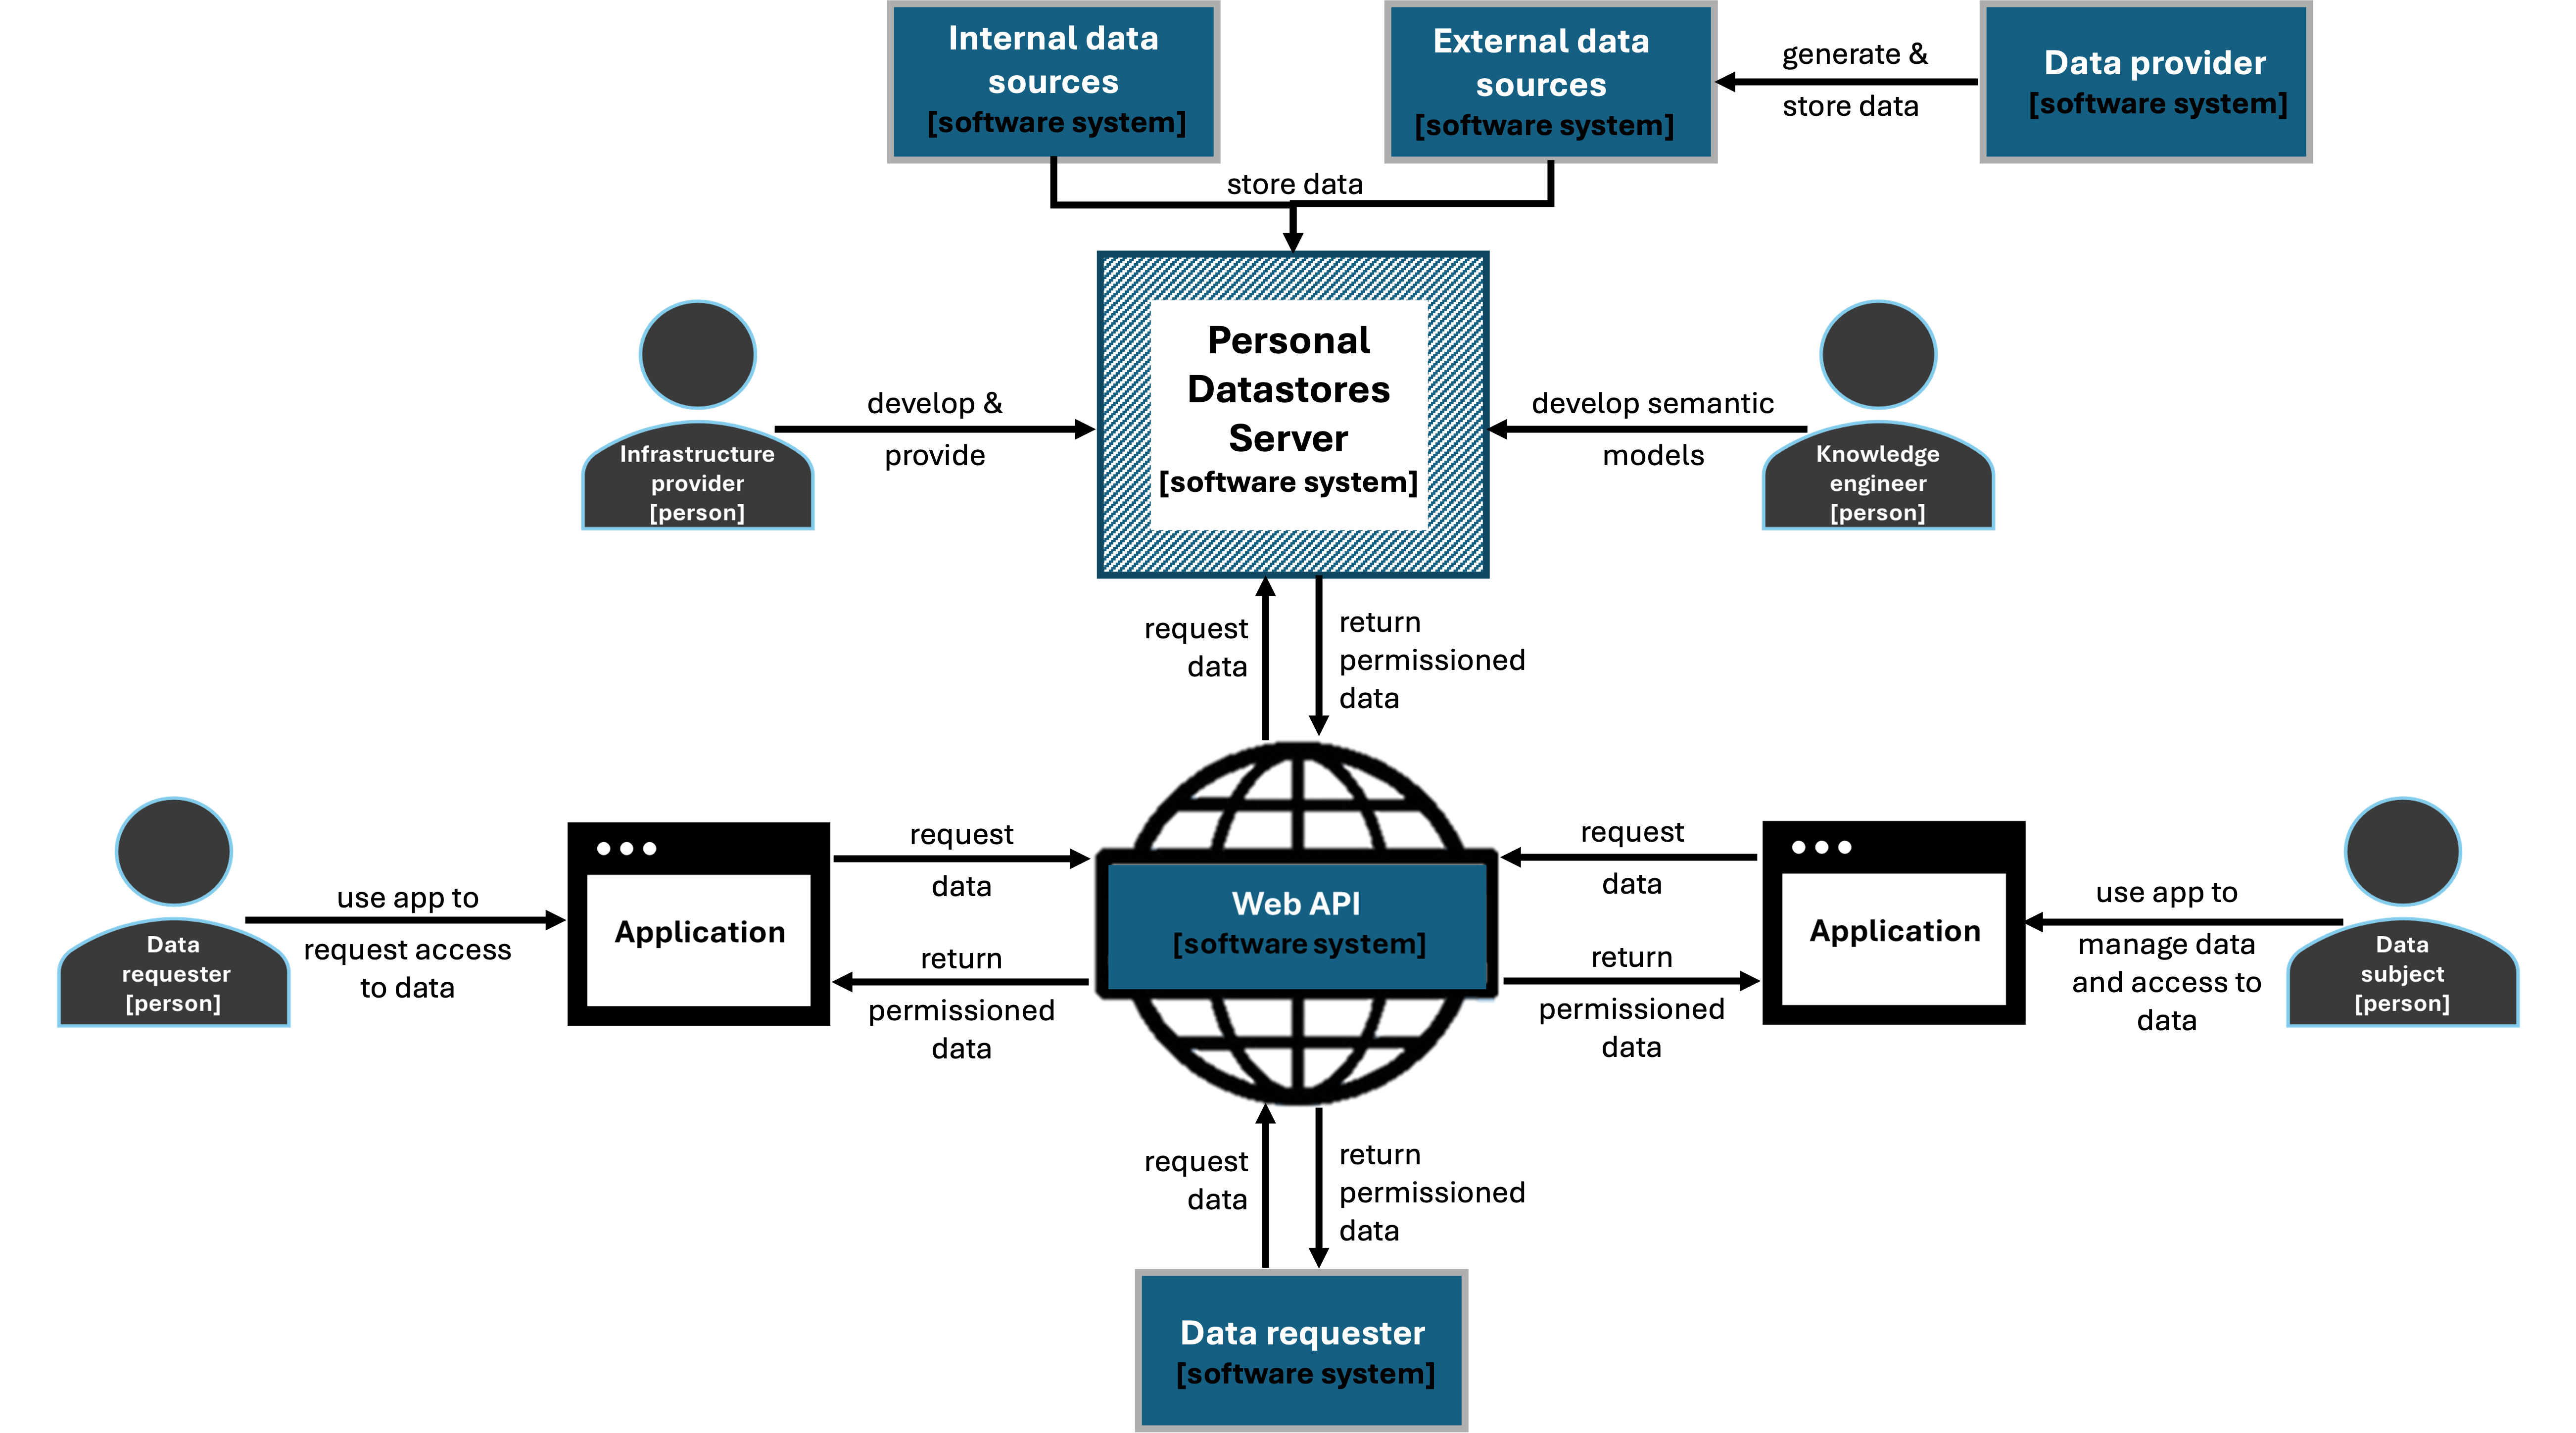
\includegraphics[width=1\linewidth]{figures//chapter-6/system-context-diagram.png}
    \caption{System context diagram of a decentralised data sharing ecosystem.}
    \label{fig:c4-context}
\end{figure}

In this diagram, the infrastructure provider and the knowledge engineer develop and provide services and semantic models for the main software system described in this Section, the \textit{Personal Datastores Server}.
Datastores hosted in this server are populated by internal and external data sources, such as temporal and spatial data sources, respectively.
The server also provides the access control layer of the ecosystem, allowing data requests and the return of permissioned data to be consumed by Web APIs.
Such APIs can be used by \textit{Data requesters} to consume and generate data, and also to feed Web applications that are used by individuals to request and use data.
Moreover, data subjects can also use applications to manage data and data access.


\subsection{Container modelling of a decentralised personal datastore server}
\label{sec:c4_container}

\begin{figure}[ht]
    \centering
    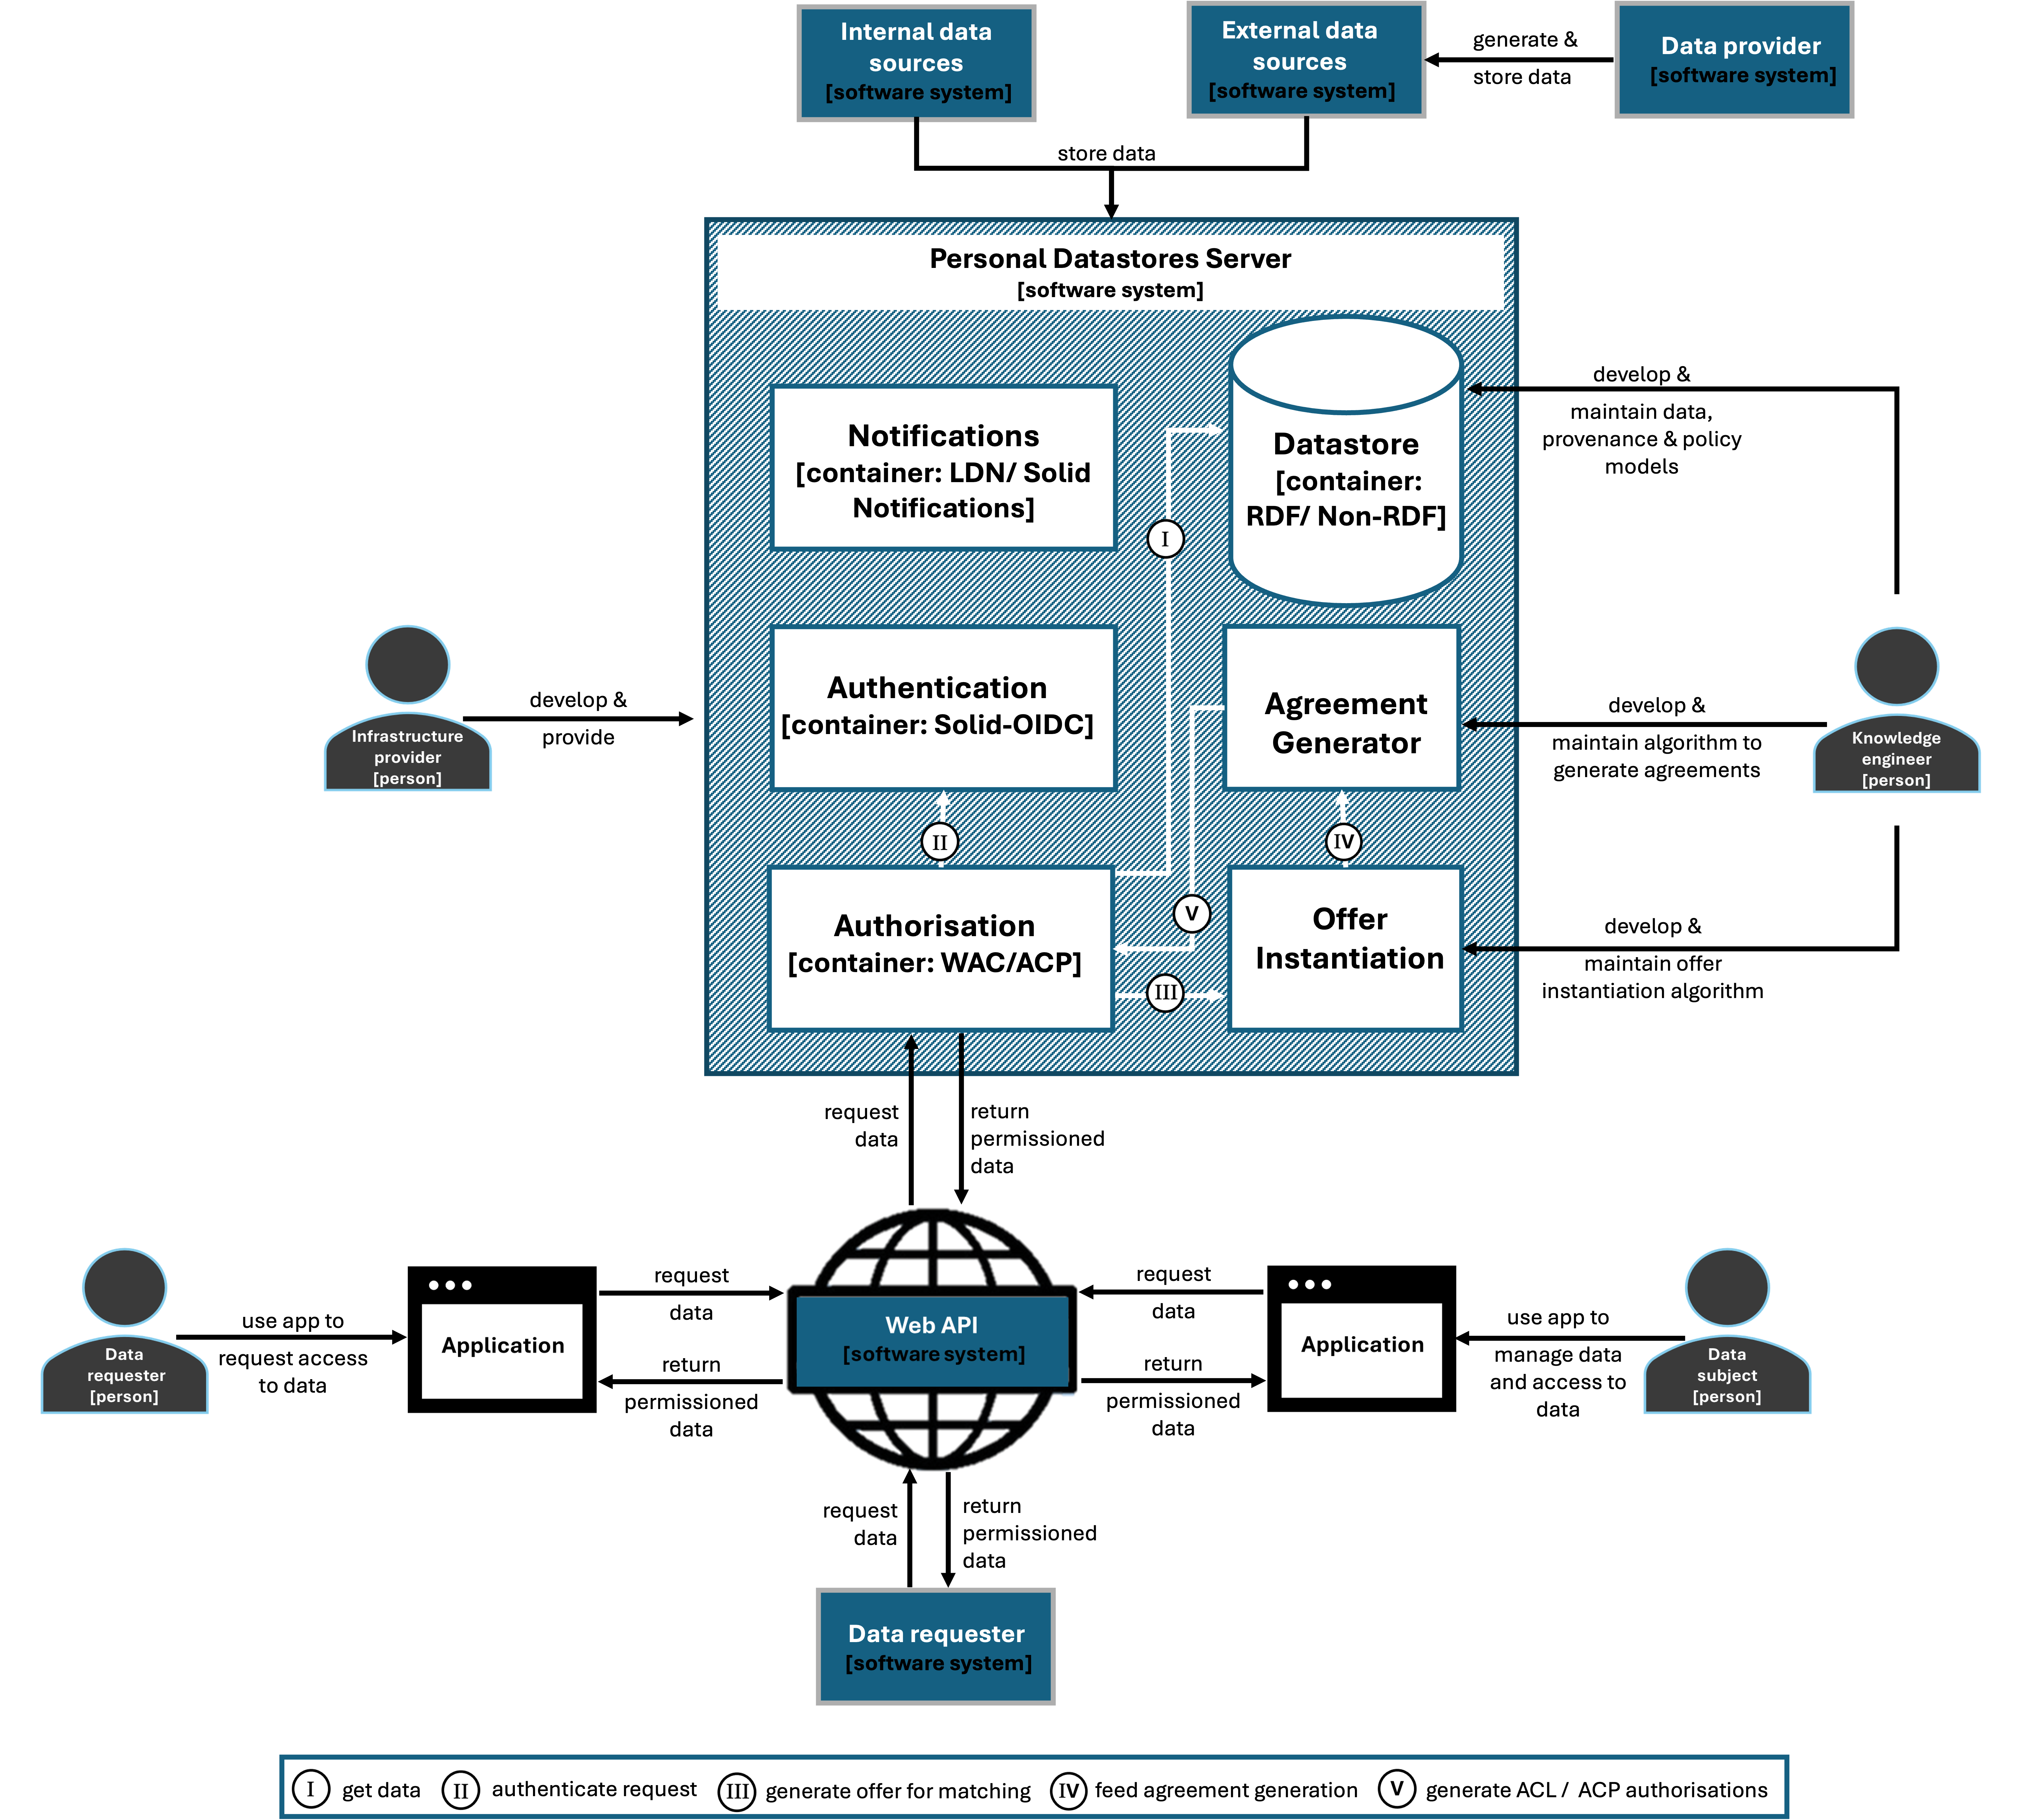
\includegraphics[width=1\linewidth]{figures//chapter-6/container.png}
    \caption{Container diagram of a decentralised personal datastore server.}
    \label{fig:c4-container}
\end{figure}

\subsection{Component modelling of a datastore and an agreement generator}
\label{sec:c4_component}

% The proposed Pod architecture, visualised in \cref{fig:architecture}, is an extension to the existing Solid Pod specification and implementations.
% We propose to add a Consent datastore component to keep a record of the consent actions already given, associated with a copy of the accepted app requests, as well as an Audit Log component to store metadata related to logins, access requests, changes in policies and consent authorisations and so on.
% In this context, the permissions and prohibitions specified by the users or the contents of the policy matching, described above by the algorithm in \cref{fig:implementation}, can be considered as the consent of the user.
% Moreover, the recording of informed consent is performed as followed: (i) the controller requests for consent through an access policy request; (ii) the Pod matches the request with the stored user policies; (iii) in the case where a match is found, the application UI presents the user with a message such as \textit{`\textbf{Application X} wants to access \textbf{data Y} for \textbf{purpose Z}. This request matches your preferences to allow access to \textbf{data Y} for \textbf{purpose Z}. Grant or refuse access?'}, and otherwise a similar message will be displayed without the matching user preference; and (iv) the user's choice in consent is stored and used in further access control requests solicited by the application in question.
% Automatic authorisations can also be performed over the matching of user preferences and apps policies, however this cannot be considered as informed consent.
% For instance, taking into consideration the requests in \cref{lst:request-registration} and \cref{lst:request-research}, the application should specify that \cref{lst:request-research} requires explicit consent from the user since it is directly related to sensitive categories of data, while \cref{lst:request-registration} is related to email and social networks information and therefore automated authorisation can be permitted.

% The existing Notification Mechanism should also be updated to allow for update or revoke requests regarding consent and the Reasoner component should be extended to be able to reason over ODRL policies stored on the ACL files.

% The User Interface, along with the Authentication and Inbox features already provided by the existing Solid specification, proposes the addition of two components: Metadata and Policies Editors.
% These components will assist users to craft granular policies for the management of access to their Pod, without burdening them with technicalities of writing ODRL policies.
% The proposed Service client should also implement an Inbox feature for the notification mechanism already discussed and additionally a Policies Editor for the crafting of access permission requests based on the proposed ODRL profile.